\documentclass[11pt]{article}
\sloppy

\usepackage{graphicx}
\usepackage{amssymb}
\usepackage{epstopdf}
\usepackage{fullpage}
\usepackage{comment}
\usepackage{amsmath}
\usepackage{amsthm}
\usepackage{subfigure}
\usepackage{mdwlist}
\usepackage{url}
\DeclareGraphicsRule{.tif}{png}{.png}{`convert #1 `dirname #1`/`basename #1 .tif`.png}


%\usepackage{lineno}

%\linenumbers

\textwidth = 6.9 in
%\textheight = 9 in
\oddsidemargin = 0.0 in
\evensidemargin = 0.0 in
\topmargin = 0.0 in
\headheight = 0.0 in
\headsep = 0.0 in
%\parskip = 0.2in
%\parindent = 0.0in

\renewcommand\floatpagefraction{.9}
\renewcommand\topfraction{.9}
\renewcommand\bottomfraction{.9}
\renewcommand\textfraction{.1}

\newcommand{\ignore}[1]{}

\newcommand{\xor}{\ensuremath{\oplus}}
\newcommand{\negl}{\ensuremath{\mbox{neg}}}

\newtheorem{theorem}{Theorem}
\newtheorem{corollary}[theorem]{Corollary}
\newtheorem{lemma}[theorem]{Lemma}
\newtheorem{definition}{Definition}
\newtheorem{assumption}{Assumption}
\newtheorem{thm}{Theorem}[section]
\newtheorem{cor}[thm]{Corollary}
\newtheorem{lem}[thm]{Lemma}
\newtheorem{prop}[thm]{Proposition}
\theoremstyle{definition}
\newtheorem{defn}[thm]{Definition}
\theoremstyle{remark}
\newtheorem{rem}[thm]{Remark}
%\newtheorem{assumpt}[thm]{Assumption}

\newcommand{\nump}{\ensuremath{\ell}}
\newcommand{\nums}{\ensuremath{k}}
%\newcommand{\numm}{\ensuremath{t}}


\bibliographystyle{plain}

\title{Distributed, Threshold Signing for PKI Root}
\author{Lea Kissner \\ leak@bbn.com \and Peiter Zatko \\ mudge@bbn.com}
\date{}
\begin{document}
\maketitle

%\input{intro}
\section{Introduction}
\label{sec:intro}

In many proposals to attain BGP~\cite{bgp}
security~\cite{s-bgp1,s-bgp2,sobgp,psbgp,spv}, such as
SIDR~\cite{sidr-arch}, an address assignment authority signs resource
certificates for address spaces and autonomous system
numbers.

Ideally, a single authority would sign every resource certificate. A
single signer could easily ensure that the signed certificates did not
conflict; for example, no two certificates would assign the same
address space to different parties. However, political considerations
seem to preclude this solution in the case of
address space and autonomous system number resource certificates.

An alternate solution involves each of the five regional internet
registries (RIRs) acting as independent certificate authorities. Each
RIR would agree to sign certificates only for their own address
space. Unfortunately, this approach is far more complex in practice:
preventing accidental address space allocation overlap or accidental
removal of address allocations across multiple RIRs is hindered in
such a stove-piped solution.  In addition, at least five public keys
(one for each RIR) must be distributed to and updated by all
verifiers. While verifiers must obtain and trust some public key in
order to verify the validity of certificates, increasing the number of
necessary trust anchors greatly increases the complexity of the system
for verifiers and can reduce security.

In order to obtain many of the benefits of a single signing authority
while allowing the RIRs to retain their autonomy, in this paper we
outline procedures to allow multiple players to operate a single {\it
virtual} signing authority as a {\it root collective}. This virtual
signing authority would have a single public key, making it appear as
a single signing authority to verifiers, but signing would be
cooperatively performed by some subset of the players. The RIRs appear
to be operationally suitable to form the root collective. We
illustrate the process of creating a signature in
Figure~\ref{fig:sign-combine}.

The virtual signing authority must be:
\begin{itemize}
\item {\bf Secure.} If the private (signing) key is leaked or
otherwise obtained by an adversary, that adversary can sign erroneous
data. We refer to such keys as {\it compromised}. The virtual signing
authority must be at least as secure as a single signing authority,
including the ability to utilize existing hardware security modules
for protection of the secret key. In fact, our scheme for a virtual
signing authority can be considered more secure, as more than one
secret key must be leaked in order to break the scheme.

\item {\bf Invisible.} No verifier should need to know the
administrative arrangements of the certificate signing
system. Signatures on certificates are verified from a single trust
anchor just as if there was a single signing authority instead of a
virtual signing authority.

\item {\bf Efficient.} Signing certificates should not be a heavy
burden on the members of the root collective. In particular, the
amount of interactive communication during signing should be minimal:
one player distributes data to be signed and the other players return
{\it signature shares}, which can be combined into a complete signature,
valid under the virtual signer's public key. In addition, our scheme
for a virtual signing authority can actually increase availability
over a single signer, because not all players in the root collective
must be available to produce a signature.
\end{itemize}

\ignore{

\begin{figure}
\begin{center}
\fbox{
\begin{minipage}{5in}
\centerline{
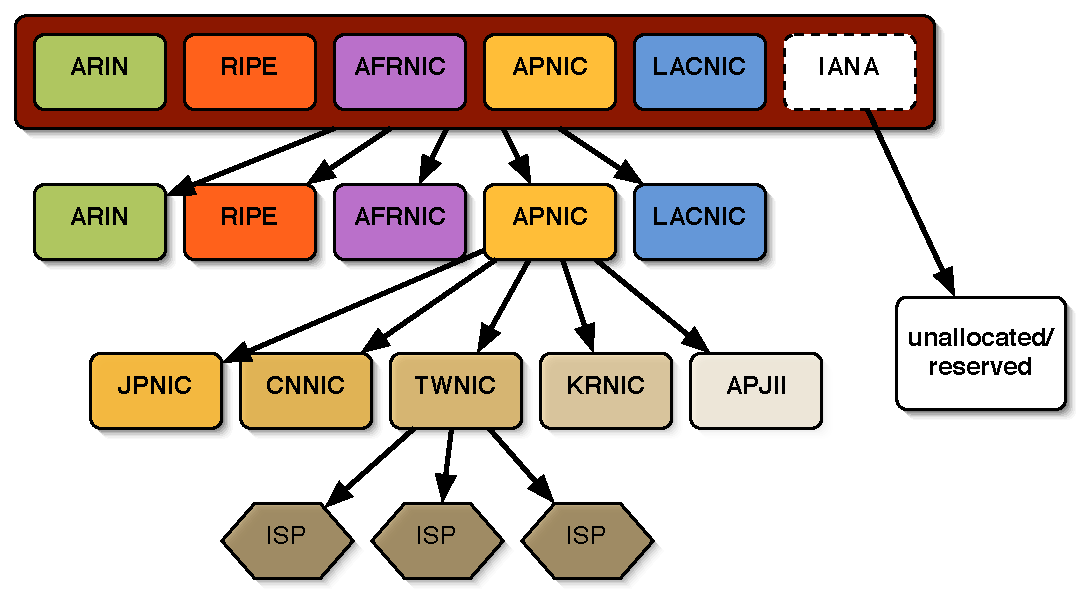
\includegraphics[width=5in]{figures/pki-hierarchy} 
}
\end{minipage}

}% FBOX
\end{center}
\caption{\small The address PKI root should be managed by the five RIRs in collaboration with IANA. The root of the hierarchy signs certificates allowing each RIR to securely manage its allocated address space. Each RIR, in turn, signs certificates for the address allocations of  ISPs and/or country registries, who may delegate sections of the address space in turn.}
\label{fig:hierarchy}
\end{figure}

}

\begin{figure}
\begin{center}
\fbox{
\begin{minipage}{5in}
\centerline{
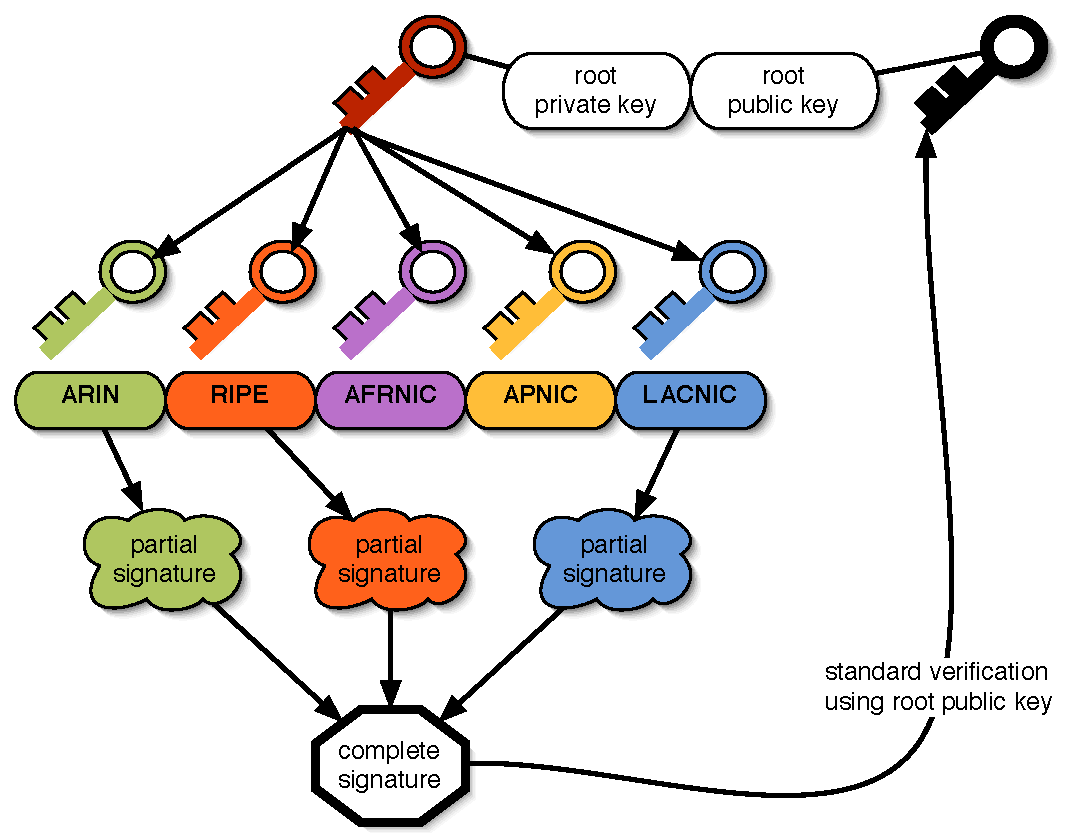
\includegraphics[width=5in]{figures/sign-combine} 
}
\end{minipage}

}% FBOX
\end{center}
\caption{\small The distributed root of a PKI functions as follows:
(1) a trusted dealer chooses a root public and private (signing) key;
(2) the dealer creates shares of the signing key for each player/RIR;
(3) to create a signature, at least $\nums=3$ players create signature
shares from their key shares and combine them into a complete
signature; (4) the complete signature can be verified with the root
public key, just as if it were created directly from the root private
key.}
\label{fig:sign-combine}
\end{figure}

\section{Concept and Operation of a Distributed Root}
\label{sec:operation}

The root of a PKI signs certificates for its subordinates; in turn,
these subordinates may sign certificates for subordinates of their
own\footnote{Subordinates may issues certificates only if they are
permitted to do so by being specified as a certificate authority in
their X509 certificate.}. The root public key acts as the ultimate
trust anchor within the proposed PKI. As such, it is an extremely
tempting target for attack. In a scenario where multiple parties
represent the public key, the security of the root private key can be
increased by employing a threshold signature scheme to split the root
private key among several players. Quorums of root collective members
distributed over the globe collectively act as the root signing entity
by jointly signing data to be verified with a single root verification
key. Thus the RIRs are responsible for managing address allocations
and certificates without requiring IANA to engage in such day-to-day
operational issues.


All \nump\ participants in the root collective jointly generate key
shares for
 each player such that $\nums\leq \nump$ players must
collaborate to
 sign data; no group of fewer than $\nums$ players can
sign data. (See Section~\ref{sec:overview} for details.) At any later
time they can sign data as
 follows: any \nums\ players individually
construct shares of the
 signature using their key share; any
computer may then combine these
 signature shares into a valid
signature under the root key.

Splitting the root signing key in this way protects against up to
$\nums-1$ players being compromised or attempting to cheat. In
combination with strong physical security, the root collective can
achieve robust protection of the root signing key while simultaneously
distributing control among the participants. To protect against
undetected compromise of root collective participants, we recommend
they refresh their key shares as we discuss in
Section~\ref{sec:refresh}. Use of threshold signature can also
increase availability, as $\nump-\nums$ players may be unavailable or
slow in response without hindering the signature process.

\ignore{To increase their ability to detect a cheating or corrupted player of
the root collective, the players may employ proofs of
correctness. Along with his signature share, each player also
constructs a small proof that his share was correctly
constructed. Some players, however, may wish to use cryptographic
hardware that cannot generate such proofs. The scheme remains secure
even in the absence of these proofs; it is only somewhat harder to detect a
cheating or corrupted member of the root collective.}


This paper is a companion to software (see Appendix~\ref{sec:code})
that performs key generation, signing, and verification according to
Victor Shoup's threshold RSA signature scheme~\cite{shoup-sig}. In
addition, we have added the capability to perform key refresh
as we outline in Appendix~\ref{sec:proof-refresh}. Operated according to
the procedures described in this document, this code performs the core
tasks necessary for a collective of players to operate a virtual
signing authority.

\input{overview}
\input{keygen}
\input{use-box}
\input{how-sign}
\input{refresh}
\section{Conclusion}


To increase both availability and security of a PKI root, a collection
of responsible parties may share the root signing key between
them. They must carefully and jointly generate the key in order to
ensure that each gains a secret share of the signing key. When data
must be signed, the requesting player sends it to all other
players. Those players then decide whether it is valid data that
should be signed. If it is, the players each create a signature share
from that data and their secret key share and return the signature
share to the requesting player. The requesting player then combines
the signature shares into a complete RSA signature valid under the
root signing key. In order to guard against the known or unknown
compromise of signature shares, the root collective should refresh
their key shares periodically. Key refresh allows the players to
obtain new key shares without changing the public key. Given the
logistical and security issues surrounding public key distribution,
key refresh allows more practical recovery compromise of a small
number of key shares.


\vspace{.25in}
{\bf Acknowledgments:} We would like to thank Steve Kent for his
insightful comments as well as Derrick Kong and Charlie Gardiner for
their help in software testing.


\bibliography{pki}


\appendix

\input{notation}
\input{proof}
\section{Detailed Key Generation Procedures}
\label{sec:keygen-detail}

In this section, we detail a list of requirements and procedures for
the trusted ceremony official and the participants.

The trusted official will be provided with the software required to
load onto a laptop and perform the key generation in advance of the
meeting. Each member will be given copies of the software in advance
and will be permitted to verify that the software that the trusted
official will load is the same as the software that they were provided
for review.


The trusted official provides:
\begin{itemize}
\item A generic laptop computer with CD-ROM drive and USB
connection\footnote{USB is presented as an example option for
removable media. If there are security concerns regarding USB devices,
the participants could elect to use one-time recordable CD-ROMs or any
other mutually agreed upon media.}, but without a hard disk.

\item Software CD-ROM with the requisite OS loader and software that the
trusted official will use and that can be examined by the participants
prior to start.
\item (optional) Hardware key generation device, such as SafeNet Luna PCMCIA.
\end{itemize}

{\noindent Each representative from the root collective provides the following:}
\begin{itemize}
\item A suitably equipped laptop with a CD-ROM drive
\item A USB flash drive
\item A RSA public key on either a CD-ROM or USB flash drive (this key
pair must be generated only for this ceremony; the corresponding
private key must be secret)
\end{itemize}

Once the official and RIR representatives verify that all participants
are present and have brought the appropriate resources, setup may
commence. All hardware should not be connected to any physical
network, have all wireless capabilities turned off or removed, and
should remain under the owners' control at all times.

Each representative from the root collective boots their system. They
are then provided with the CD-ROM containing the software that the
trusted official will be using\footnote{The CD-ROM should be {\bf
read-only}, alternatively the trusted official can make multiple
copies of the CD-ROM in front of everyone (6 in this example), provide
a CD-ROM to each participant and retain the final copy for use.}. The
participants are permitted to copy the CD-ROM, examine its contents,
and perform any checksum operations they feel necessary to foster a
strong belief that the contents of the CD-ROM are correct and
consistent with what they had previously been provided.

The official boots their system from the software CD-ROM, which
contains a bootable linux kernel that runs in RAM only.  Additionally,
the CD-ROM contains the required software for key generation, key
share splitting, handling the key shares, and
sanitization. Sanitization software clears system memory and prevents
aversaries from utilizing forensic capabilities to retrieve any
portions of the private key shares.

The official loads each of the public keys presented by the members of
the root collective onto the system.  After this is accomplished the
trusted official generates a new RSA public/private key pair and
subsequently, using a software application, splits the RSA private key
into key shares. The joint secret key is then destroyed. The key
shares, one for each member of the root collective, are encrypted
using the corresponding player's public key. The resulting encrypted
key shares and root public key are loaded onto their respective USB
memory sticks and returned to their owners. After the keys have been
transferred, the sanitization software is executed to remove any
remaining traces of the private key or private key shares from the
official's system and the system is powered down.


\ignore{



The trusted official brings the following to the ceremony:
\begin{itemize}
\item Laptop computer with CD-ROM drive and USB connection, but no disk drive or network connection
\item Bootable CD with a RAM-drive-based Linux distribution and key generation/splitting software
\item (optional) Hardware key generation device, such as a SafeNet Luna PCMCIA
\end{itemize}

{\noindent Each member of the root collective brings the following to the ceremony:}
\begin{itemize}
\item A USB flash drive or CD containing an RSA public key, at least as strong as the key generated in this ceremony, generated for the occasion (the corresponding private key remains at the RIR's headquarters)
\item (optional) A laptop with CD-ROM drive, suitable for copying the software CD and examining the code on it
\end{itemize}

{\noindent The ceremony then proceeds as follows in the presence of the root collective. At any point any member of the root collective may object to the security of the proceedings and stop the key generation ceremony.}
\begin{enumerate}
\item The trusted official presents the laptop for inspection; the laptop may not be touched by anyone other than the official, but he can open it and perform requested tests.
\item The trusted official lets the members of the root collective copy the software CD (using the laptops they brought for the purpose) and examine the software. (Members of the root collective may examine the software later, as well. If they find a problem, they may object to the root key being used.)
\item If a hardware key generator is being used, it is attached to the system. 
\item The trusted official boots the laptop from the software CD-ROM (using a RAM disk) and loads the system.
\item The trusted official generates a new RSA public/private key pair. (We discuss hardware key generation on SafeNet's Luna products in Appendix~\ref{sec:hardgen}.)
\item Using a software application, the trusted official splits the RSA private key into key shares, one for each member of the root collective, and destroys the private key corresponding to the root public key.
\item For each player, the trusted official inserts a player's USB flash drive, uses the public key loaded on that drive to encrypt that player's secret key share, then copies the encrypted key share and the root public key  to the flash drive. 
\item The trusted official runs a cleanup application and powers down the key generation laptop. (If the laptop has other memory in it, such as a writable BIOS, the cleanup application or further action must be taken to erase the contents of that memory.)
\end{enumerate}

}
\input{code}
\section{API and Implementation Details}

 \subsection{Hardware Key Generation}
\label{sec:hardgen}

While hardware key generation entails greater logistical and security complexity, they can generate cryptographic keys using better entropy sources than available on most computers. The following directions were provided by SafeNet for SafeNet's Luna line of hardware security modules\footnote{This information is courtesy of Robert
Woodward, Alan Boyd, Mark Yakabuski, and Ben Hanrahan at SafeNet,
Inc.}:
\begin{enumerate}
\item Generate the key using the PKCS call {\tt C\_GenerateKeyPair(... CKM\_RSAX\_9\_31\_KKEY\_PAIR\_GEN, ...}, as this mechanism is FIPS approved
\item Extract the private key from the hardware device. \\
	{\tt C\_GenerateKey( ... CKM\_AES\_KEY\_GEN, ... pTemplate)} (This should set the {\tt CKA\_WRAP} and {\tt CKA\_DECRPYT} attributes to true and returns the handle of the AES key used to wrap the RSA key.) \\
	{\tt C\_WrapKey(... CKM\_AES\_CBC\_PAD, wrapping key handle, handle of key to wrap)} (This returns  the wrapped key blob.) \\
	{\tt C\_DecrypInit(... CKM\_AES\_CBC\_PAD, wrapping key handle)} \\
	{\tt C\_Decrypt(... wrappedKeyBlob, ... , pData, ...)} ({\tt pData} will not contain the decrypted key in DER-encoded form.)
\end{enumerate}
Note that in order to export a key, the key export bit must be set on the hardware generation device. Once set, this bit cannot be cleared without wiping the device. Thus, we recommend using a separate device than the ones used for signing by the root collective.

\subsection{}
\label{sec:use-box-detail}

Players can import a secret key into SafeNet's Luna devices as follows\footnote{This information is courtesy of Robert
Woodward, Alan Boyd, Mark Yakabuski, and Ben Hanrahan at SafeNet,
Inc.}:
\begin{enumerate}
\item Generate a 3DES or AES wrapping key on the HSM with both it's
{\tt CKA\_ENCRYPT} and {\tt CKA\_UNWRAP} bits set

\item DER encode (PKCS\#8) the RSA key and encrypt it ({\tt
C\_Encrypt}) on the HSM with the wrapping key; this call returns the
encrypted blob

\item unwrap via {\tt C\_Unwrap} the encrypted blob on the HSM using the same
wrapping key; this call returns the key handle of the imported RSA key
\end{enumerate}
The public key may be imported into the HSM using the {\tt
C\_CreateObject} call from PKCS\#11.

From this point, the player may create signature shares as standard
RSA signatures using the secret key in the HSM.


\end{document}
